\documentclass[tikz, border=10pt]{standalone}
\usetikzlibrary{shapes,arrows,positioning}

\begin{document}
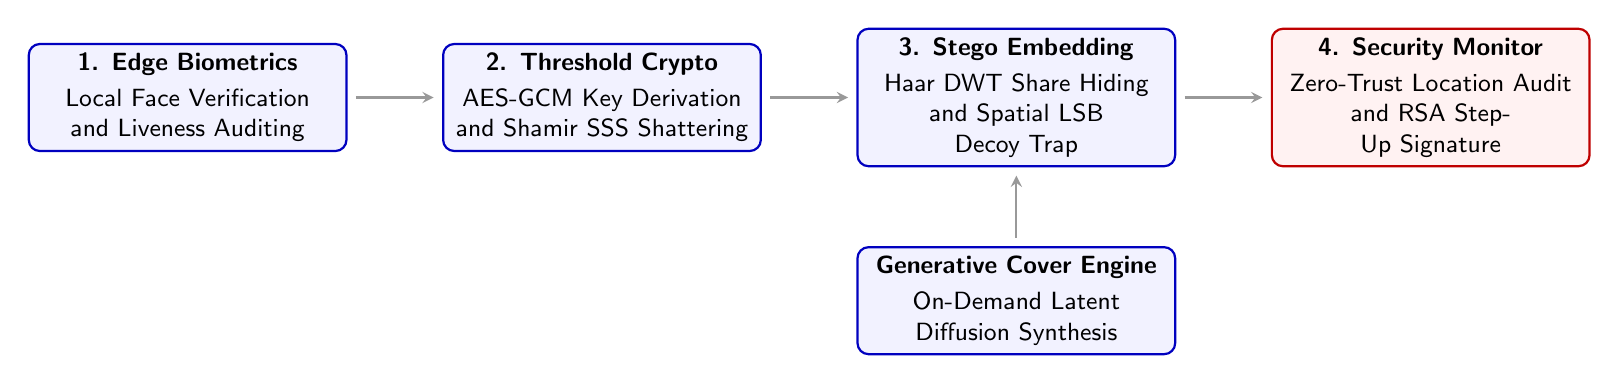
\begin{tikzpicture}[
    node distance=1.0cm and 1.2cm,
    auto,
    block/.style={
        rectangle,
        draw=blue!75!black,
        thick,
        fill=blue!5,
        text width=3.8cm,
        align=center,
        minimum height=1.3cm,
        rounded corners=4pt,
        font=\small\sffamily
    },
    block_accent/.style={
        rectangle,
        draw=red!75!black,
        thick,
        fill=red!5,
        text width=3.8cm,
        align=center,
        minimum height=1.3cm,
        rounded corners=4pt,
        font=\small\sffamily
    },
    line/.style={
        draw,
        -stealth,
        thick,
        shorten >=3pt,
        shorten <=3pt,
        draw=gray!80
    }
]

    % --- Nodes (Horizontal Flow with robust par-spacing) ---
    \node [block] (biometrics) {
        \textbf{1. Edge Biometrics} \par\vspace{2pt}
        Local Face Verification \\ and Liveness Auditing
    };
    
    \node [block, right=of biometrics] (crypto) {
        \textbf{2. Threshold Crypto} \par\vspace{2pt}
        AES-GCM Key Derivation \\ and Shamir SSS Shattering
    };
    
    \node [block, right=of crypto] (stego) {
        \textbf{3. Stego Embedding} \par\vspace{2pt}
        Haar DWT Share Hiding \\ and Spatial LSB Decoy Trap
    };
    
    \node [block, below=of stego, node distance=1.5cm] (generative) {
        \textbf{Generative Cover Engine} \par\vspace{2pt}
        On-Demand Latent \\ Diffusion Synthesis
    };
    
    \node [block_accent, right=of stego] (monitor) {
        \textbf{4. Security Monitor} \par\vspace{2pt}
        Zero-Trust Location Audit \\ and RSA Step-Up Signature
    };
    
    % --- Flow lines ---
    \path [line] (biometrics) -- (crypto);
    \path [line] (crypto) -- (stego);
    \path [line] (generative) -- (stego);
    \path [line] (stego) -- (monitor);
    
\end{tikzpicture}
\end{document}
